% Data Model
\begin{figure}[htb]
    \centering
    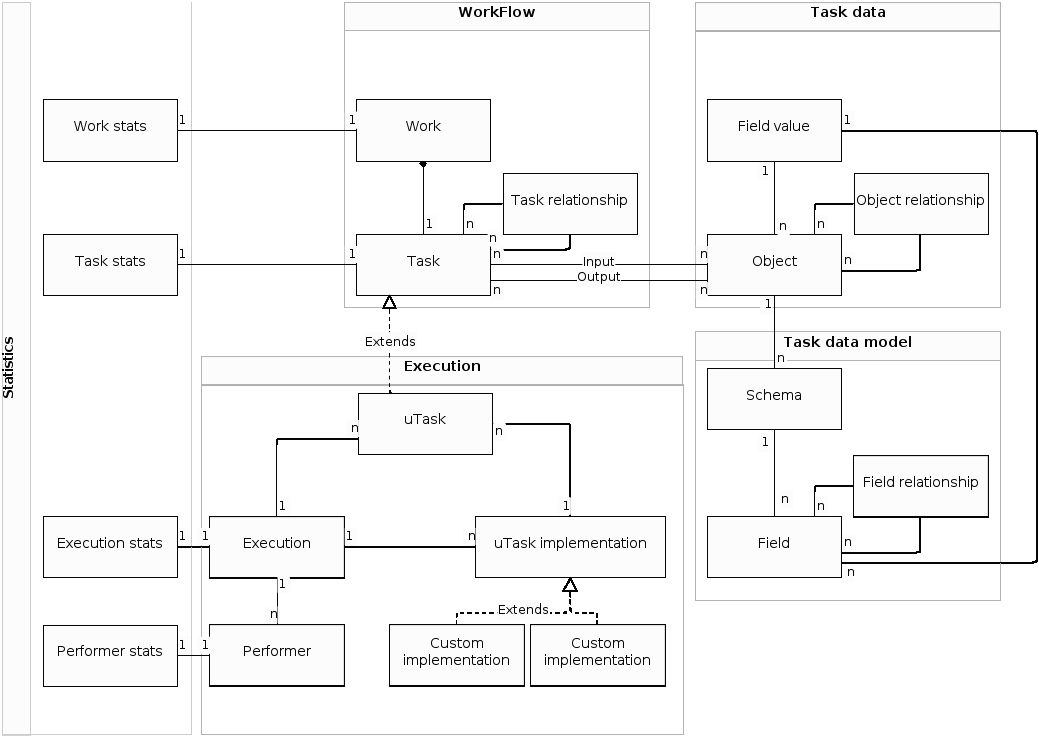
\includegraphics[width=\columnwidth]{DataModel}
    \caption{Overall Data Model schema, with logical subdivision.}
    \label{fig:data-model}
\end{figure}
\begin{figure}[htb]
    \centering
    
\includegraphics[width=0.75\columnwidth]{ConceptualModel}
    \caption{Conceptual organization of Work, Task and \utask{}.}
    \label{fig:conceptual-model}
\end{figure}

% task con custom proiperties in modo da configurare i runtime

% Step su come funziona la creazione di un task

% Schema type?
% Input data can be associated with a set of Properties, i.e. name-values pairs that have a domain-specific meaning (e.g. the validation status of a given Tweet to be analysed)


% Strategies???

\subsection{WorkFlow}
The WorkFlow embodies all the data associated to the \emph{flow} of Task
that need to be executed in order to complete a set of Tasks. The tasks can belong
to different archetypes (e.g. Human, Automatic) and have their own set of assigned
objects. The \emph{Workflow} is composed of:
\begin{description}
    \item[The Work:] is the abstract representation of a set of Tasks related
    to each other.
    \item[The Flow:] describes how the Tasks, belonging to a Work, are related
    to each other, also defining the type (e.g. dependency, parallel) of relation
    between such Tasks. 
    \item[The Task:] is the representation of a general activity that can be
    performed by the framework.
\end{description}

\subsubsection{The Work}\label{data:work}
The \emph{Work} represents a set of related Task finalized to the execution of
some kind of data manipulation or analysis on a set of input Objects. The
result of the execution produces output Objects described by a Schema. The Work
is defined by:
\begin{itemize}
    \item A \textbf{Name} that identifies the Work.

    \item \textbf{Constraints} used to bind some aspect of the Work or to make
    decision for giving less or more priority to this work with respect to the
    others. Example of constraints are: Due date, Performer skills, Max execution
    time, etc.

    \item \textbf{Input} data, defined by a \emph{Schema} and the associated
    Objects. To keep the model as general as possible no assumption are made on
    the \emph{Schema} type (relational, graph, etc.).
    \item \textbf{Output} data, defined as an extension of the input schema
    (sharing the same schema type).

    \item A set of \textbf{Task} composing the Work. Their orchestration is made
    at design time, by specifying a \emph{Flow}.
\end{itemize}

\subsubsection{The Task}
The Task is the central unit of computation, It represent a single activity
focusing on a particular action. The activity must not be an atomic operation,
like in an algorithm a single function call, but it should be focused on a
single purpose. For example tagging an image can be considered as a single Task,
otherwise tagging and validating an image should be divided in two separated
tasks if possible. the flexibility of the framework allow the creation of any
type of Task, the previous statement is only an advice to better separate
different activities into different Task. As we mentioned our system can
seamlessly handle complex Task involving multiple activities, such as whole
\ac{GWAP} game into a single Task. A Task is characterized by:
\begin{itemize}
    \item A \textbf{Name} that identifies the Task.

    \item \textbf{Input} data, defined by a \emph{Schema} and the associated
    Objects. To keep the model as general as possible no assumption are made on
    the \emph{Schema} type (relational, graph, etc.). Usually the Schema
    is a projection of the Schema of a Work. Like the Schema the input Object
    usually are a selection of the Work input Objects.
    \item \textbf{Output} data, defined as an extension of the input schema
    (sharing the same schema type).

    \item A Task \textbf{type}\footnote{An assumption is made to make the list fit
    all the possible abstract task our framework is able to handle.}
    defining, at abstract level, what kind of data manipulation will be performed
    by a Task. These categorization are taken from \cite{paperboz}, here are a
    few:
        \begin{itemize}
            \item Like
            \item Order
            \item Classify
            \item Add
            \item \omissis
        \end{itemize}
    \noindent Each Task type is defined by:
        \begin{itemize}
            \item I/O relationship, defining, at abstract level, how the Task
            transforms the data and the schema.
            \item A default implementation.
        \end{itemize}

    \item A \textbf{Status} encoding the current state of the Task. A Task, can
    have only one of the following statuses at point of its lifecycle:
        \begin{itemize}
            \item \emph{Planning-Input}: the Task has been created, have a
            \emph{Schema} and \emph{Object data} associated and a defined Task
            \emph{type}.

            \item \emph{Planning-\utask{}}: a set of \utask{} has been associated
            to the Task.
            
            \item \emph{Planning-Assignment}: a set of \emph{Performers} has
            been selected to execute the \utask{}.
            
            \item \emph{Wait}: Task planned, \utask{} ready for execution.
            
            \item \emph{Running}: \utask{} are running.
            
            \item \emph{Ended}: all the \utask{} have completed their execution.
        \end{itemize}
    
    \item A set of \textbf{Subscriber}s able to receive updates on the Task
    execution. The Subscribers are declared during the Task creation step and the
    updates that they will receive are about change on the Status of the Task.

    \item A set of \textbf{Execution constraints} used for prioritizing the Task
    among others or to modify the standard behavior of the Task. The constraints
    that can be used are the same defined for the Work in \ref{data:work}.

    \item \textbf{Configuration data} are application specific data used to
    configure the behavior of the Task once it is executing. For instance
    we can store here the classes for a classify Task type.

    \item \textbf{\utask{}}s are the instances of Task assigned to one or more
    Performers on a Device, to be performed on one or more input Objects.
    % TODO ???

    \item An \textbf{Aggregation} function, in charge of collecting the \utask{}
    results and generate the Task output.
    
    \item \textbf{\utask{} planning} strategy, in charge of defining how many
    \utask{} create for a given Task and associate the right portion of input
    objects to each \utask{}. For example total disjunction, redundancy, partial
    overlap, etc.
    
    \item \textbf{Performer assignment} strategy able to assign \emph{Performers}
    to \utask{}. Some strategies can be: manual, random, most reliable, etc.

    \item \textbf{\utask{} implementation} strategy in charge of routing the
    correct \utask{} implementation for each \utask{} execution. The routing
    can be \emph{fixed} for everyone, can be done according to the
    \emph{user-agent} (e.g. Browser) or other conditions.

    \item A \textbf{Task planning} which embodies the functionalities of
    \emph{\utask{} planning} strategy, \emph{Performer assignment} strategy and
    \emph{\utask{} implementation} strategy and whose purpose is to decide the 
    logic behind the invocation of those strategies.

    \item A \textbf{Task control} strategy is able to control the status of the
    Task and if needed perform corrective actions.

    \item An \textbf{Emission policy} specifying which \emph{Subscriber} need to
    be notified of a Task change in \emph{Status}.
\end{itemize}


The \textbf{relationships} that may exist between Tasks are materialized into the
\emph{Task Relationship} object. This object contains all the information related
to the flow of the task execution during the execution of a Work. An example of
a Task relation can be the validation of the results obtained by an Automatic
computation task previously performed. In this case the relation is the simple
sequence.

In a flow we can use \emph{Control Structures} and \emph{Variables}. The
\emph{variables} are included into the flow to control the behavior of the Work
and can be modified by some condition upon Task execution. For instance if an
Automatically obtained results from Task are below a certain threshold, this
check is performed after the Task execution, then a variable is changed accordingly.
The \emph{Control Structures} are common to all the Workflow managers and 
control hoe the Tasks are executed:
\begin{description}
     \item[Sequence:] represent the normal flow of an application where one
     operation is executed after the previous is completed.
     \item[Choice:] give the possibility to made choice according to one, or
     more, \emph{Variables}.
     \item[Loop:] Allow to execute some steps multiple times, according to a
     predefined value or a \emph{Variable}.
     \item[Parallel:] the steps of the flow are not executed in \emph{Sequence},
     allowing the parallelization of some steps.
 \end{description} 









\subsection{Task Data Model}
The Task Data Model contains all the information about the Task metamodel. The
metamodel is organized in Fields and the Fields are grouped into a Schema. This
data structure resembles the standard DBMS schema organization, where we have
a Schema defined as a collection of Fields with possible relationship between
them. The Task Data Model is composed by
\begin{description}
    \item[The Schema:] is the abstract representation of a table structures.
    \item[The Field:] contains all the information of the field type and
    relationships.
\end{description}


\subsubsection{The Schema}
The Schema is used as a container of Fields that compose the metamodel of the
Task data. The Schema is defined by:
\begin{itemize}
    \item A \emph{Name}

    \item A \emph{list of Fields} defining the structure of the Task data.

    \item A \emph{list of Objects} representing the Task Data instances
\end{itemize}

The Schema is in \textbf{relation} with the actual data instances of the Task,
called Objects, and the Fields it is composed of.


\subsubsection{The Field}
The Field contains information on the type of the data it contains and information
on the relation between two, or more, Fields (like the type of dependency).
The Field is composed by:
\begin{itemize}
    \item A \textbf{Name} that identifies the Field.
    
    \item A \textbf{type} defining the type of the data that this field contains,
    for instance \code{string}, \code{number}, etc.

    \item A set \textbf{related fields}. the relationship between the fields
    is defined by the \emph{relation} attribute.
    
    \item A \textbf{relation} that specifies which type of relationship occurs
    among the \emph{related fields}.

    \item The \textbf{list of field values} representing the data contained within
    this field in the Object structure.
\end{itemize}

The \textbf{relationship} existing between the Field are materialized using the
\emph{Field Relationship} table. Here we have all the information of the fields
involved and on the type of the relationship (e.g. derivate of, copy of, calculated
etc.).








\subsection{Task Data}
The Task Data contains the actual data instance for each Task, defined in the
\emph{Schema}. All the data are contained in a \emph{Object} that represent the
the instance of the Task data (e.g. A row of the Task Data table). Due to the
metadata-like model of the System, we need to store all these information into
a separate table and use the \emph{Object} as a simple reference table.

\subsubsection{The Object}
The Object contains the actual data value as reference to field value instances;
it's composed by:
\begin{itemize}
    \item A \textbf{Name}.
    \item A list of field values \textbf{data}.
    \item TODO ??
\end{itemize}


\subsubsection{The Field Value}
The Field Value contains the data associated to a particular field, defined in
the metedata model. It's defined by:
\begin{itemize}
    \item An \textbf{Object} that define tho what \emph{Object} they refer to.
    \item The \textbf{Field} to which the data belongs.
    \item TODO ???
\end{itemize}







\subsection{Task Execution}
The Task Execution embodies all the information relative to the actual execution
of the code. The majority of these data belongs to the \textbf{Execution layer}
thus can be physically located into another piece of software in charge of the
execution of the code.


\subsubsection{\utask{}}
The \utask{} is the implementation of a Task that insist on a specific subset
of data of the Task. Can be also considered as an activity assigned to one or
more Performers. It is defined by:
\begin{itemize}
    \item A \textbf{Name}.
    
    \item A list of \textbf{Execution}, representing the actual activities
    performed by a \emph{Performer}
    
    \item A set of \textbf{Execution constraints}.
    
    \item \textbf{Input} data, as a subset of the Task input data.
    
    \item \textbf{Output} data, with the same schema as the related Task output
    data.
    
    \item A list of \textbf{Properties}, defined as name-value pairs, having
    domain specific meaning. 
    
    \item One or more \textbf{\utask{} implementation}.
\end{itemize}







\subsubsection{The Execution}
The Execution is related to one \emph{Performer} that need to compute a \utask{}.
An Execution is defined by:
\begin{itemize}
    \item a \textbf{Status} telling the status of the execution of the \utask{},
    the available statuses are:
    \begin{itemize}
        \item \emph{running}
        \item \emph{suspended}
        \item \emph{idle}
        \item \emph{ended}
    \end{itemize}

    \item A set of \textbf{Execution data} provided as \ac{JSON} object.

    \item A \utask{} \textbf{Implementation}
\end{itemize}







\subsubsection{\utask{} implementation}
The \utask{} Implementation is the actual application logic and presentation
delivered to a \emph{Performer} to run a \utask{}. The System provides a default
implementation according to the Task type, in addition, a \emph{Requester} can
specify one or more Custom implementations, in order to obtain more control over
the execution process.








\subsubsection{Performer}
A Performer is a human being able to execute one or more \utask{}. The performer is characterized by a set of attributes such as:

\begin{itemize}
    \item A \textbf{Name}
    \item \textbf{Demographic} information
    \item \textbf{Performance} information
    \item \textbf{Trustworthiness}
    \item \textbf{Social properties}
\end{itemize}






\subsection{Statistics}
This Statistics model contains all the information related to the Task profiling
and statistics used to tweak the performance of a Task, or used by components
(like the \emph{Task controller}) to take decision on the Task flow. In this
model are contained data about \emph{Work}, \emph{Task}, \emph{\utask{}},
\emph{Performer}, etc. The data contained in these tables can be:
\begin{itemize}
    \item \textbf{Creation date}
    \item \textbf{Total execution time}
    \item \textbf{Average number of \emph{Performer}s per hour}
    \item \textbf{Last execution}
    \item etc.
\end{itemize}
